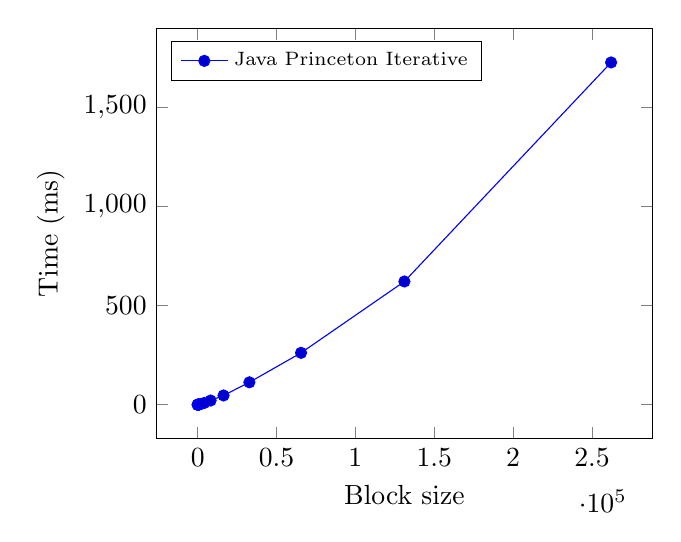
\begin{tikzpicture}
\begin{axis}[xlabel={Block size},ylabel={Time (ms)},width=0.65\linewidth,legend pos=north west,scaled y ticks = false,legend cell align=left,legend style={font=\scriptsize}]
\addplot coordinates {
(16, 0.1398)
(32, 0.0492)
(64, 0.1078)
(128, 0.1991)
(256, 0.3547)
(512, 0.7740)
(1024, 1.7228)
(2048, 3.8546)
(4096, 8.8053)
(8192, 21.1757)
(16384, 46.8150)
(32768, 113.1953)
(65536, 261.9954)
(131072, 622.4328)
(262144, 1728.4640)
};
\legend{Java Princeton Iterative}
\end{axis}
\end{tikzpicture}
